\documentclass[12pt]{report}
\pagestyle{headings}
\usepackage{rotating}
\usepackage{graphicx}
\usepackage{longtable}
\usepackage[tt]{titlepic}
\usepackage{verbatim}
\setlength{\parindent}{0.0in}
\setlength{\parskip}{0.1in}
%\setcounter{secnumdepth}{1}
%\setcounter{tocdepth}{1}

%\addtolength{\textheight}{2cm}
%\addtolength{\footskip}{2cm}

\newcommand\placeholder[2]{
	\noindent
	{\setlength{\fboxsep}{0pt}
		\makebox[#1]{
			\parbox{0pt}{\rule{0pt}{#2}}
			\parbox{#1}{
				\centering
				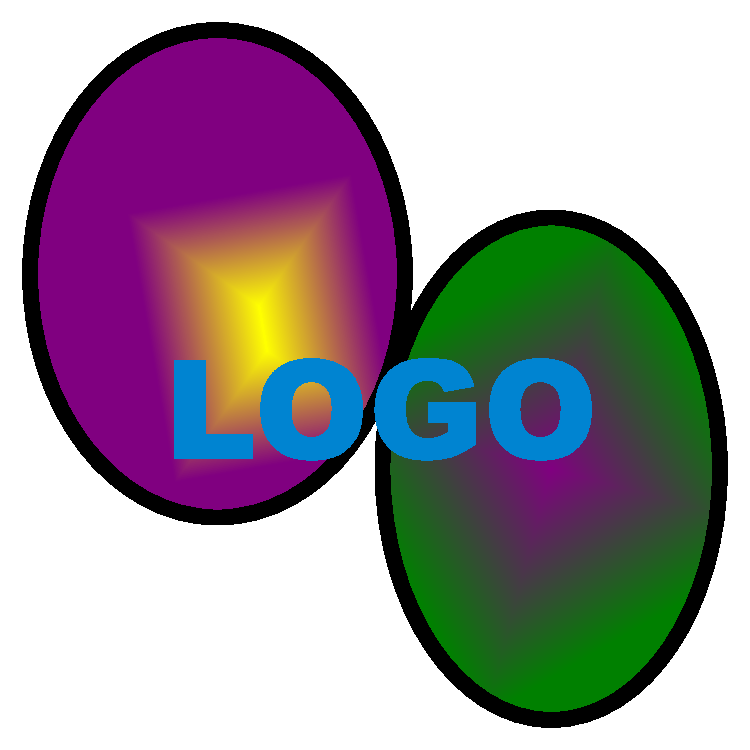
\includegraphics[width=0.50\textwidth]{logo.ps}
			}
		}
	}
}

\author{Holger Ludvigsen,\\Vegar Neshaug,\\Jon Skarpetveit,\\Rahele Zarabi,\\Kristoffer Selboe}
\title{{\small Eksperter i Team\\TPG4850 VR-Landsbyen}\\\textbf{Team 4 (V.I)}}
\date{{\small \today}}
\titlepic{\placeholder{\textwidth}{0.5\textwidth}}

\begin{document}
\maketitle

\pagenumbering{roman}

As a part of the course Experts in Team (EiT) at NTNU, five students were put in a group to collaborate on a project. This team (us) was a part of the virtual reality village of EiT, and came up with the following problem statement:

\begin{center}\em How can you make an affordable and usable prototype\\for head tracking to be used for virtual reality?\end{center}
\vspace{\parskip}

We solved this problem by first doing a preliminary study followed by design and imlementation of the solution. In the preliminary study, several technical and theoretical subjects were investigated. The mathematics behind estimation of object position from pictures were elaborated. We looked at the available technology for connecting a high definition camera to a PC and reading the images from it. We studied the properties of infrared light. We checked out and tested the Nintendo Wii and its Wiimotes. Lastly, potential areas of use for a solution was described.

Then, a specification of the requirements was carefully crafted. The specification was the basis for the design of the solution. This design specifies how the components of the system is constructed and how they are connected. The components of the system make up a pipeline:

\begin{figure}[h]
\centering
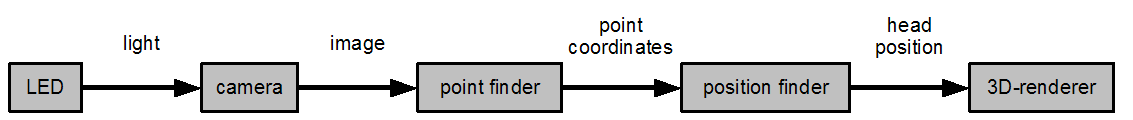
\includegraphics[width=\textwidth]{graphics/main_design_english.png}
\end{figure}

The LED-component is a set of infra red LEDs that are attached to the user's head. These transmit light that is captured by a high definition camera. The image from this camera is read by a point finder software that attempts to locate the coordinates of the bright dots in the image where the LEDs are. These coordinates are transferred to the position finder software which uses them to estimate the position of the user's head. This head position is then used by the 3D-renderer software to display a 3D-scene on a screen where the viewpoint is mapped to the head position.

Course
Project group
Problem statement
Prestudy
How solved:
	Reqspec
	Design
	Implementation
Result
Evaluation
Conclusion
\pagebreak
	
\setlength{\parskip}{0.0in}
\renewcommand*\contentsname{Innhold}
\tableofcontents
\renewcommand*\listtablename{Tabell-liste}
\listoftables
\renewcommand*\listfigurename{Figurliste}
\listoffigures
\chapter*{Akronymliste}
\pagebreak
\setlength{\parskip}{0.1in}

\renewcommand*\chaptername{Kapittel}
\renewcommand*\partname{Del}

\pagenumbering{arabic}
\setcounter{page}{1} % start normal page counting here

\chapter{Innledning}

	\chapter*{Introduksjon}

\chapter{Forstudie}

	\section{Matematikken bak trackingen (Vegar)}

	

\section{Tilkobling av kamera til PC}

	For � koble et kamera til en PC og lese dens videobilder trenger man b�de maskinvare og programvare. Maskinvaren gir den fysiske tilkoblingen mellom kameraet og PC-en samt gj�r lavniv�s logikk og behandling av dataene. Programvaren abstraherer bort maskinvaren og gir utviklere et brukbart grensesnitt for � lese og bruke videobildene. Av maskinvare har vi i prosjektet tenkt � bruke HDMI og et Intensity-kort for � koble kameraet til PC-en som kj�rer systemet v�rt. Av programvare har vi tenkt � bruke DirectShow for � f� lett tilgang til videobildene fra kameraet.
	
\subsection{HDMI og Intensity}

	HDMI er en standard for et fysisk grensesnitt for � sende og motta digital lyd og bilde. Apparater med HDMI-kontakt kan kobles til hverandre ved hjelp av en HDMI-kabel (se figur \ref{fig:hdmi}). HDMI er designet for � h�ndtere lyd og bilde med h�y oppl�sning, og kan sende opptil 10,2 gigabit per sekund.
	
	\begin{figure}[h]
	\centering
	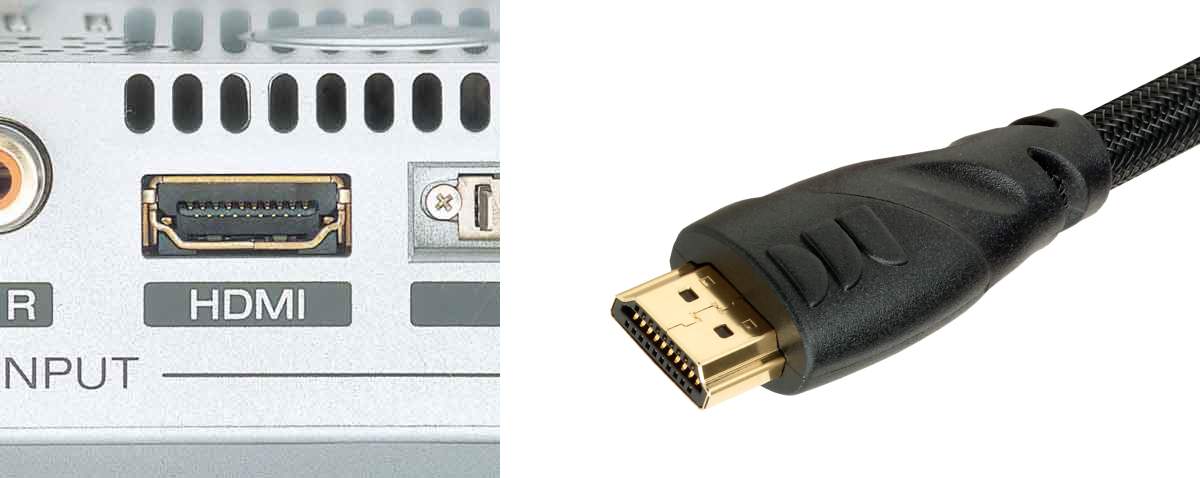
\includegraphics[width=0.60\textwidth]{graphics/hdmi.png}
	\caption{HDMI-kontakt (venstre) og kabel (h�yre)}
	\label{fig:hdmi}
	\end{figure}
	
	Intensity er et HDMI capture card fra Blackmagic Design. Det er et stykke maskinvare som kan settes inn i en PC for � gj�re det mulig � koble enheter til denne PC-en gjennom HDMI. Kortet kobles til PCI-express-porten i PC-en og har to HDMI-kontaktpunkter: inngang og utgang (se figur \ref{fig:intensity}).
	
	For � kunne f� ut bilde fra HD kameraet trengte vi HDMI input port som overf�rer data i en s� stor hastighet slik at vi slipper � komprimere bildestr�mmen. Vi valgte Blackmagic Intesity card som gir den beste og siste teknologien innen HDMI til Windows eller Mac OS. Intesity kortet har en HDMI inngang for HD kameraer som gir den h�yeste kvalitet p� bilde. HDMI kan lese ukomprimert bildestr�m direkte fra kameraet. Bildestr�mmen er i 1080i (interlaced) det vil si at bilde har en oppl�sning p� 1920 x 1080 piksler. 1080 linjer i vertikal retning og 1920 linjer i horisontal retning. Interlaced betyr at kameraet tar opp bilder med et alternerende sett med linjer slik at oddetallslinjene og partallslinjene oppdateres annenhver gang. Det vil si at det trengs to oppdateringer for � skape et fullstendig bilde, man �ker bildekvaliteten av et videosignal uten � �ke b�ndbredden. N�r bildet skal vises p� skjerm utf�res det en deinterlacing som er en teknikk for � konvertere interlaced bildestr�m til progressive bildestr�m. Hvis det er 1080p (progressive) trenger bildestr�mmen kun � oppdateres en gang for � f� et fullstendig bilde, at alle linjene vertikalt blir skannet ved en oppdatering. 
	 
	\begin{figure}[h]
	\centering
	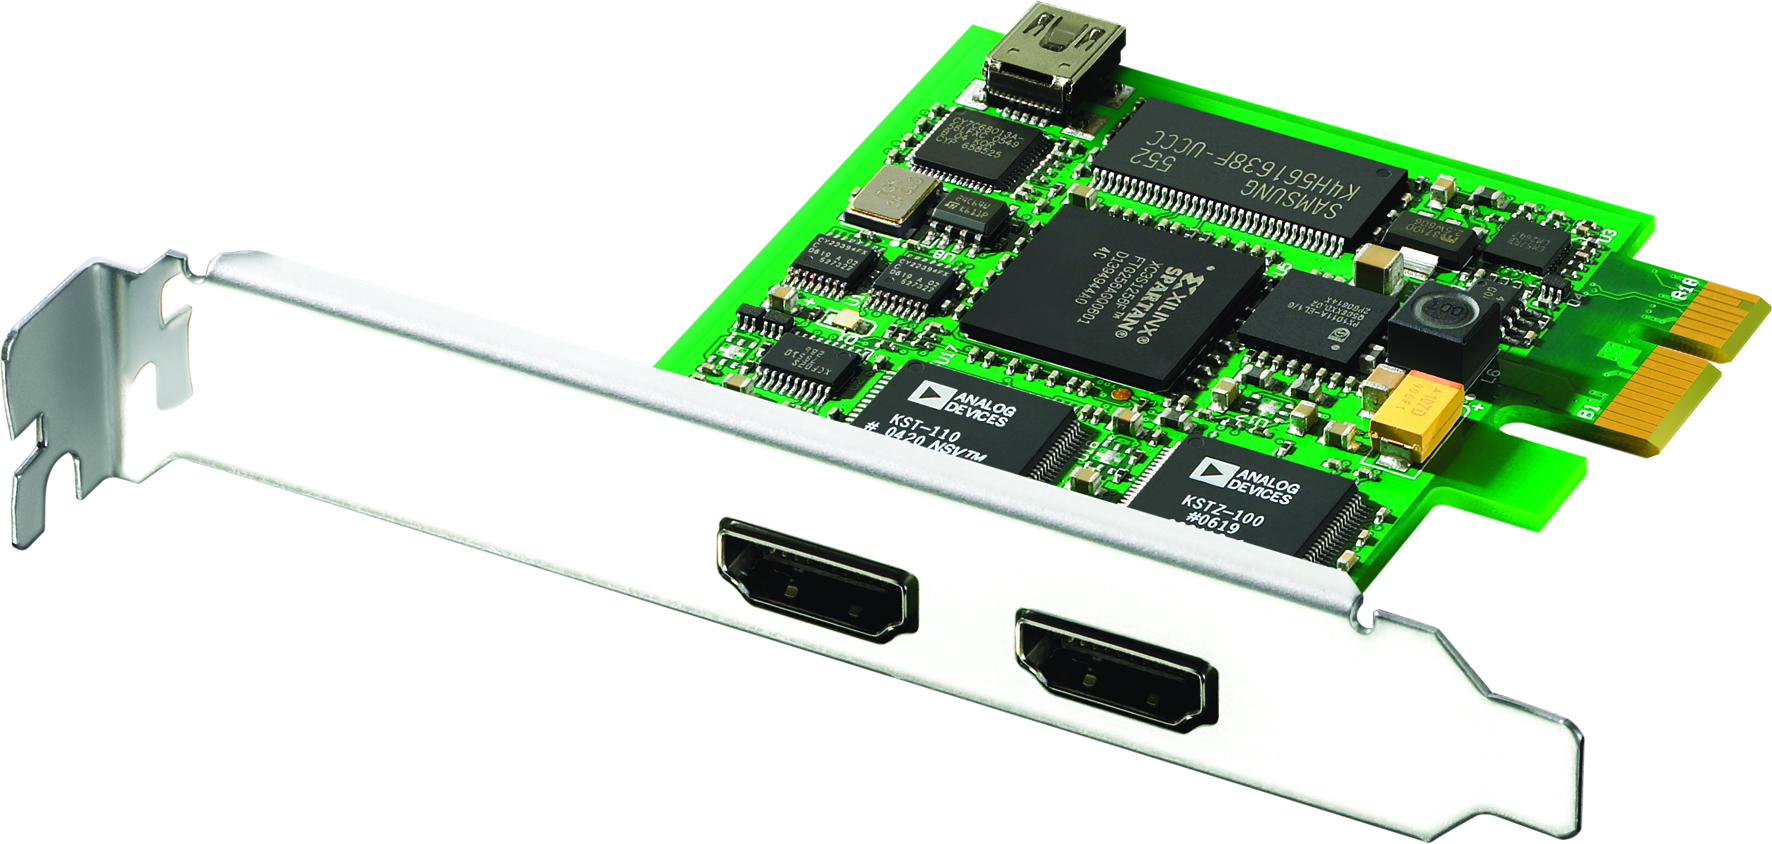
\includegraphics[width=0.60\textwidth]{graphics/intensity.png}
	\caption{Intensity fra Blackmagic Design}
	\label{fig:intensity}
	\end{figure}

\subsection{DirectShow}

	DirectShow er et rammeverk og programvaregrensesnitt for � h�ndtere multimedia p� PC-er. Det er utviklet av Microsoft og gj�r det mulig � spille av og ta opp media (typisk lyd og/eller bilde) gjennom et felles grensesnitt, og abstraherer bort maskinvaren. Bildene fra videokamera koblet til et Intensity-kort er tilgjengelig gjennom DirectShow. DirectShow er tilgjengelig gratis fra Microsofts nettsider.
	
\subsection{Infrar�dt lys}

	Infrar�d lys er elekektromagnetisk str�ling av b�lgelengder lengre enn b�lgelengdene til synlig lys. Det synlige lyset har b�lgelengder mindre enn 750nm. Ordet infra kommer fra latinsk og betyr under, og r�d er den fargen innenfor det synlige spekteret som har den lengste b�lgelengden. Det infrar�de lyset som ligger n�rmest det synlige lys har mye av de samme egnskapene som det synlige lyset bortsett fra at det er usynlig for det mennesklige �yet. Infrar�dtlys er derfor mye brukt til blant annet overv�kning og nattkamera, i tillegg til ignaler i elektriske kontroller. Infrar�d str�ling med lengre b�lgelengder er mer knyttet til varmeproduksjon og varmesensitive kameraer som er mye brukt i romfartsindustri og v�penindustri.

	I dette prosjektet er det en fordel � bruke infrar�dt lys fordi et lyspunkt som er synlig for det mennesklige �yet kan v�re forstyrrende for brukeren og det kan blande seg med andre lyskilder i omgivelsene rundt som vil gj�re det vanskligere finne punktene vi �nsker under prosesseringsarbeidet. 
	
\section{Nintendo Wii og Wiimotes}

	Nintendo Wii er en spillkonsoll som ble lansert i 2006. I stedet for realistisk grafikk fokuserer den p� alternative former for styring av spill. Wiimote er navnet p� kontrolleren som brukes for Wii. Se figur \ref{fig:wiimote}. Det er en tr�dl�s kontroller med infrar�dt kamera og akselerasjonsmeter. Innebygd er det maskinvare som kalkulerer bildekoordinater til filmede infrar�de lys og sender disse via et tr�dl�st nettverk (Bluetooth).
	
	\begin{figure}[h]
	\centering
	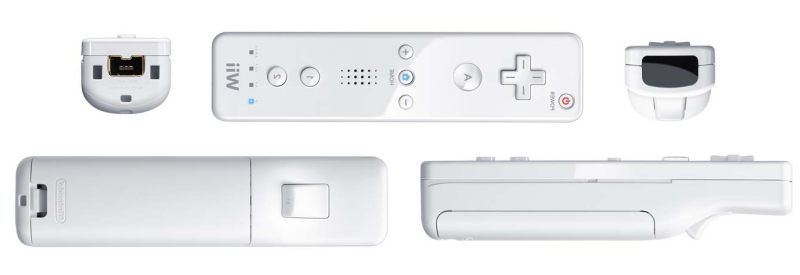
\includegraphics[width=0.60\textwidth]{graphics/wiimote.png}
	\caption{Nintendo Wiimote}
	\label{fig:wiimote}
	\end{figure}

\section{� spore punkter i et bilde (Holger)}

	

\section{Bruksomr�der (Jon)}

	

\chapter{Kravspesifikasjon}

		I dette kapitlet spesifiseres kravene til systemet som skal utvikles. Kravene er delt inn i funksjonelle og ikke-funksjonelle krav. Funksjonelle krav beskriver hva et system er i stand til � gj�re. De spesifiserer ikke kvaliteten, effektiviteten eller implementasjonen av disse funksjonene. Med andre ord, the sier \emph{hva} en bruker kan gj�re med systemet. Ikke-funksjonelle krav beskriver egenskaper ved systemet som ikke er direkte funksjoner. De er relatert til systemet som en helhet. Tabell \ref{table:f_req_spec} og \ref{table:nf_req_spec} viser de funksjonelle og ikke-funksjonelle kravene til systemet som skal lages.
	
	\begin{table}[h]
		\centering
		\begin{tabular}{| c | c | p{9 cm} |}
			\hline 
			\bf ID & \bf Prior. & \bf Description \\
			\hline
			\hline
			FR1 & H�y & Systemet skal spore posisjonen til et menneskehode i tre dimensjoner. \\
			FR2 & H�y & Den sporede posisjonen skal oppdateres n�r hodet beveger p� seg. \\
			FR3 & Lav & En tre-dimensjonal scene skal vises p� en skjerm foran menneskehodet hvor kameraposisjonen i scenen er lik posisjonen til hodet i rommet. \\
			\hline
		\end{tabular}
		\caption{Funksjonelle krav}
		\label{table:f_req_spec}
	\end{table}
	
	\begin{table}[h]
		\centering
		\begin{tabular}{| c | c | p{9 cm} |}
			\hline 
			\bf ID & \bf Prior. & \bf Description \\
			\hline
			\hline
			NFR1 & H�y & Prisen for systemet skal v�re under 10 000 NOK. \\
			NFR2 & Lav & Eventuelt utstyr brukeren m� ha p� seg skal v�re lettere enn 300 gram. \\
			\hline
		\end{tabular}
		\caption{Ikke-funksjonelle krav}
		\label{table:nf_req_spec}
	\end{table}
	
\chapter{Design og implementasjon}

	\section{Design av l\o sningen}

	

\section{Implementasjon av l\o sningen}

	

\chapter{Resultat og evaluering}

	\section{Resultatet av prosjektet}

	

\section{Evaluering av prosjektet}

	

\chapter{Konklusjon og videre arbeid}

	VR-landsbyen har v�rt veldig resultatorientert, og oppgavene har kun v�rt innenfor datateknologi. Gruppa v�r har fungert meget bra n�r det gjelder samarbeidsprosessen, men vi har hatt en del problemer med oppgavel�sningen. Problemene kom av gruppas manglende datakompetanse. Dette har naturlig nok f�rt til en del frustrasjon, men vi er glade for at dette ikke har f�rt til noen interne konflikter i gruppen. Vi har ubevisst rettet v�r frustrasjon utad istedenfor innad i gruppen. 

Vurderingen v�r av gruppen er at vi p� de fleste omr�der har fungert som et godt team. Ett ankepunkt er kanskje mangel p� beslutningsdyktighet. Vi f�ler ikke at gruppa er satt sammen av den riktige faglige kompetansen for � kunne l�se de oppgavene som ble lagt fram i VR- landsbyen optimalt. �Men samtidig mener vi man som profesjonell skal kunne fungere i et team som best�r av medlemmer med tverrfaglig bakgrunn. Gjennom dette prosjektet har vi sett at vi likevel klarte � f� til ganske mye, og at vi tilegnet oss mye ny l�rdom. Dette gj�r at vi neste gang ikke vil se like m�rkt p� en vanskelig oppgave hvor vi mangler viktige forkunnskaper. 
� 
N�r det gjelder samholdet og trivselen i gruppa, har den hele veien v�rt veldig god. Samholdet har holdt seg like godt b�de i medgang og motgang, og dette har ogs� syntes godt utad. Dette har blant annet v�rt takket v�re sosial sammenkomst og teambuilding fra fasilitatorene og landsbyleders side. Dette f�rte til �kt selvtillit og viljen til � st� p� ble merkbart bedre etter dette. 

Vi har i Eksperter i Team ikke f�tt noen erfaringer i � jobbe med personer som er vanskelig � samarbeide med. Vi har heller ikke opplevd andre store konflikter under gruppearbeidet. Vi har derimot h�stet erfaring i hvordan en gruppe p� best mulig m�te kan utnytte de resursene som hvert enkelt gruppemedlem utgj�r og kunnskapen de besitter. Vi har sett at det er viktig � kartlegge de enkeltes sterke sider p� et tidlig tidspunkt slik at disse kan komme gruppen raskt til gode. Vi har gjennomf�rt adferdstest og satt oss inn i en del gruppeteori som vi ikke har reflektert noe s�rlig over ved tidligere teamarbeid. Vi synes alle at vi har f�tt bedre innblikk i hvordan vi selv opptrer i et team. Vi tror erfaringene v�re fra EiT vil gj�re oss mer bevisste p� teamprosess ved senere prosjekter og i arbeidslivet. 


\appendix

	\chapter{TODO: Appendix here}

\pagestyle{plain}
\pagebreak
\pagenumbering{roman}
\setcounter{page}{1} % end normal page counting here

\chapter{Ordliste}

	\begin{description}
	\item[1080i/p] At et kameras bilde har 1080 bildepunkter i h�yden og er interlaced/progressive (se interlacing og progressive)
	\item[3-dimensjonal] Se tre-dimensjonal
	\item[3D] Se tre-dimensjonal
	\item[3D-viseren] Delen av systemet som viser en 3D-scene p� skjermen
	\item[Akselerasjonsmeter] Sensor som m�ler akselerasjon
	\item[Bibliotek] Samling av kode som tilbyr nyttig funksjonalitet
	\item[Bluetooth] Type tr�dl�st nettverk
	\item[C] Et programmeringsspr�k
	\item[CCD-bildebrikke] En type brikke som kan fange et bilde til digital form
	\item[CMOS-bildebrikke] En type brikke som kan fange et bilde til digital form
	\item[Deinterlacing] � fjerne interlacing fra et bilde (se interlacing)
	\item[Diode] En type elektrisk lampe
	\item[DirectShow] Et bibliotek for � h�ndtere multimedia p� PC-er
	\item[HDMI] Et type grensesnitt for � sende digital lyd og bilde
	\item[Headsettet] Anretningen en bruker m� ha p� hodet for � bruke systemet
	\item[Intensitet] Lysstyrken til et bildepunkt
	\item[Intensity] Et stykke maskinvare for � gi HDMI-kontant til en PC
	\item[Interlacing] � sende annenhver linje av et bilde om gangen for � oppn� bedre filmkvalitet
	\item[Java] Et programmeringsspr�k
	\item[LED] Light emitting diode (se diode)
	\item[Lyspunkt] Omr�det i et bilde med h�y intensitet, sannsynligvis for�rsaket av at en lyskilde filmes
	\item[OpenGL] Et bibliotek for � vise 3D-grafikk p� PC-er
	\item[Oppl�sning] Antall bildepunkter i et bilde
	\item[PCI-express] En type tilkoblingpunkt i en PC
	\item[Piksel] Et bildepunkt
	\item[Posisjonsfinneren] Delen av systemet som finner posisjonen av hodet til brukeren
	\item[Progressive] Det motsatte av interlacing, dvs at alle linjene i et bilde sendes om gangen
	\item[Punktfinneren] Delen av systemet som finner koordinatene til lyspunktene i kamerabildene
	\item[StatoilHydro] Sponsor av VR-landsbyen
	\item[VR] Se virtual reality
	\item[Virtual reality] Simulering av virkelighet
	\item[Wii] Spillkonsoll fra Nintendo
	\item[Wiimote] Styrekontrolleren til Wii (se Wii)
\end{description}



%\nocite {a1,a2,a3,a4,a5,a6,a7,a8,a9,a10,a11,a12,a13,a14,a15,a16,a17,a18,a19,a20,a21}
\bibliographystyle{plain}	
\bibliography{literature}

\end{document}
